\chapter{FET projects and social media} \label{FET_projects_and_social_media}
This chapter focuses on the presence of FET projects on online communication channels. Section \ref{Data_set} describes the analysed sets of projects. Section \ref{Considered_channels} lists the communication channels considered for this thesis. Section \ref{Search_for_channels} outlines the search conducted to find the channels on which each FET project is active. Sections \ref{Overall_use_of_channels} and \ref{Online_presence_breakdown} provide an overview of the usage frequency of online channels made by FET projects. Sections \ref{Budget_impact} and \ref{Budget_impact_the_case_of_the_HPC_and_QT_projects} investigate the impact of the available budget on the number of online communication channels.

\section{Data set} \label{Data_set}
This thesis focuses on the online communication activity of FET projects launched within the Horizon 2020 funding scheme. The list of projects was downloaded on 15th July 2017 from CORDIS, the main portal of the European Commission on results of EU-funded research projects \cite{CORDIS}. FET projects approved after 15th July 2017 are not considered in this thesis.

The list consists of 151 projects and it is available in Appendix \ref{List_of_FET_projects}. For each project, Appendix \ref{List_of_FET_projects} reports budget and start and end date, as well as the activated online communication channels (see section \ref{Considered_channels} for the channels considered in this thesis).   

Some projects in the list were not considered for the present analysis. Excluded groups were the Flagship and Launchpad projects (see section \ref{The_FET_programme} for a brief description of the two classes), as well as projects started after 1st February 2017. Disregarded projects are listed in Appendix \ref{Specific_lists_of_FET_projects}. This procedure reduced the data set from 151 to 130 samples.

Flagship projects were not taken into account due to their budget. The funding at their disposal is far superior compared to the other FET projects, see Appendix \ref{List_of_FET_projects}. Thus, the Human Brain and Graphene Projects can invest larger resources and were not considered representative of FET initiatives in terms of communication effort. 

Launchpad projects were disregarded as their ultimate goal is to find applications of results achieved by other FET initiatives. This class of projects is characterised by limited interest in communication activities. Moreover, the available budget is relatively small (of the order of hundred thousand Euro), strongly limiting the possible communication strategy. 

Projects started after 1st February 2017 were not considered as the time span between this date and the list download was judged insufficient to fully develop and launch an adequate communication activity. The only exception is the DEEP-EST project. By the time of writing, DEEP-EST has already started a solid online communication effort.    

For some of the investigations in this thesis, the data set of 130 projects was divided into three sub-groups.  The first group consists of the 22 projects active in HPC and the transition to the exascale (see section \ref{FET_and_high-performing_computing}). The second subgroup includes the 10 projects in the field of quantum technologies (QT, see section \ref{FET_and_quantum_technologies}). The third group comprises the other 98 projects. The lists of HPC and QT projects are reported in Appendix \ref{Specific_lists_of_FET_projects}.

It must be borne in mind that the analyses presented in this thesis have been performed on small data sets. The low number of projects indicates that results show limited robustness under future changes in the data. Hence, the results reported in this work should serve as a guideline rather than as definitive statements.  

\section{Considered communication channels} \label{Considered_channels}
The communication channels offering the widest potential audience are based on the internet. Examples are websites and social media. For this reason, online channels are pillars of the FET communication strategy. 

Different approaches can be considered to assess the use of online communication channels made by FET projects. One quantitative estimate is the fraction of projects active on specific platforms. For this thesis, the following communication channels were considered:   

\begin{description}
 \item [Website] Websites are the online channels offering the highest degree of freedom. They allow the owner to personalise the content, its presentation strategy and graphic visualisation.
 \item [Facebook] Facebook is the most used social media worldwide. It offers direct interaction among users and it is mainly designed for free time.  
 \item [Twitter] Twitter is very effective for concise science-related communication. It requires high posting rates and offers less personal interaction compared to Facebook.
 \item [LinkedIn] LinkedIn is designed for professional content and enables the creation of closed groups. Nevertheless, interaction among users and outreach within the groups are limited.
 \item [YouTube] YouTube is the world's main platform for video sharing. It offers a very direct communication channel, but it is not very effective at engaging users.
 \item [Instagram] Instagram has a very active and rapidly growing community. It requires content with high visual impact and offers limited interaction among users.
 \item [ResearchGate] ResearchGate offers the possibility to share technical documentation and engage in scientific discussions with researchers. As members are mainly scientists, the reachable community is significantly smaller and more homogeneous compared to other social networks.  
\end{description}

\section{Search for channels} \label{Search_for_channels}
The analyses presented in this thesis are based on the number of FET projects considering the online communication tools mentioned in section \ref{Considered_channels}. To determine these values, a search was performed for all projects in Appendix \ref{List_of_FET_projects}. 

The search was conducted as follows. First, projects were contacted directly and asked on which channels they are active. However, in many cases it was not possible to find the contact details or no answer was received. This happened for 42 projects out of the 130 of interest for the present analysis (more specifically, for 4 out of 22 HPC projects, 1 out of 10 QT projects and 37 out of 98 other projects). A desk search was then performed to gather the required information for the 42 projects. 

It cannot be excluded that the desk search failed to find all websites or accounts activated on the social channels considered for this thesis. Thus, it is highly probable that the list of accounts in Appendix \ref{List_of_FET_projects} is incomplete. The results presented in this thesis must therefore be considered as inferior limits when describing the actual scenario. 

\section{Overall use of channels} \label{Overall_use_of_channels}
Out of the 130 projects in the data set, 124 have created a website, 66 have opened accounts on Twitter, 26 on Facebook, 20 on  LinkedIn, 13 on YouTube, 10 on ResearchGate and ... on Instagram. The results, expressed as percentage values, are reported in Figure \ref{Social_media}.

The results show that almost all FET projects have created a website. Facebook and Twitter are the two most popular social media within the FET community, hence reflecting the scenario experienced in society. Nevertheless, the fraction of projects active on Twitter is significantly larger than that on Facebook. This is opposite to what occurs in society, where Facebook is the most used social media. This indicate that Twitter is considered a more suitable tool for scientific communication. 

\begin{figure}[!t] 
 \begin{center}
 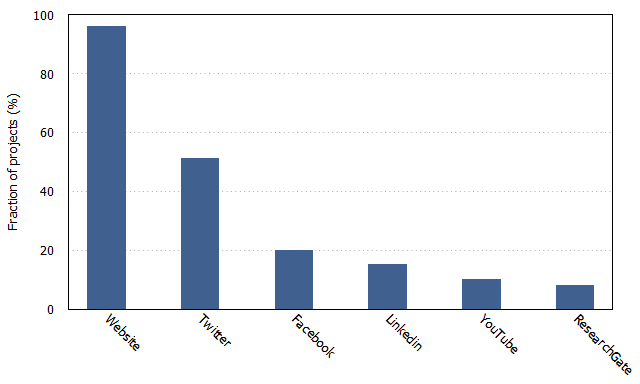
\includegraphics[scale=0.4]{Images/Social_media.png}
 \caption{Fractions of FET projects making use of the communication channels considered for this thesis.}
 \label{Social_media}
 \end{center}
\end{figure}

YouTube and Instagram are not common communication channels among FET projects. This is probably due to the difficulty of collecting content with high visual impact and suitable for drawing attention of disparate audiences not familiar with the research field. The difficulty arises from the fact that the objectives and results of FET projects are often very technical and not appropriate for image-based communication. In the case of YouTube, there is the additional complication of the resources needed for the production of high-quality videos.

The number of projects active on ResearchGate is low. This seems to indicate that ResearchGate is not seen as a suitable channel for large-scale communication activity. The reason could be the fact that the reachable audience is typically limited to researchers active in similar investigation fields.

\section{Online presence breakdown} \label{Online_presence_breakdown}
The analysis in section \ref{Overall_use_of_channels} was repeated on the projects sub-groups outlined in section \ref{Data_set}: HPC, QT and Others. This enabled a comparison of how disparate classes of FET projects make use of online communication channels. The results are shown in figure \ref{Social_media_breakdown}. 

\begin{figure}[!t] 
 \begin{center}
 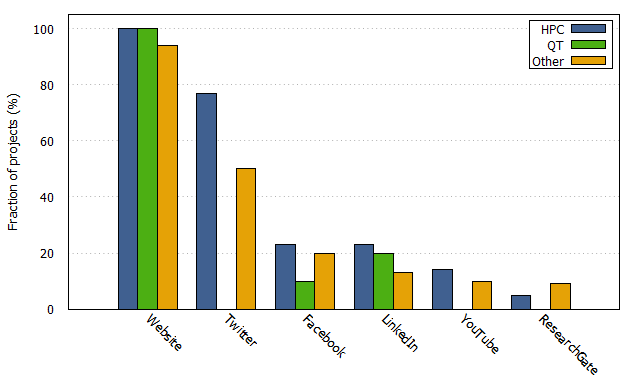
\includegraphics[scale=0.4]{Images/Social_media_breakdown.png}
 \caption{Fractions of FET projects making use of the communication channels considered for this thesis. Results are given as a function of the three project classes considered for this thesis. No QT project is active on Twitter, YouTube or ResearchGate.}
 \label{Social_media_breakdown}
 \end{center}
\end{figure}

The figure shows that basically all FET projects have created a website, regardless of the considered sub-group. As for the most used social platforms within the FET community, i.e. Twitter, Facebook and Linkedin, the HPC class has opened the most accounts compared to QT and other projects. The result indicates that HPC projects are among the most active FET initiatives in terms of online communication.  

The QT sub-group seems to follow the opposite strategy. The fraction of projects making use of social media is significantly smaller compared to HPC and other FET projects. In particular, none of them has opened an account on Twitter, the most used social platform within the FET community. 

The limited use of social media made by QT projects highlights two facts. First, the QT Flagship will design its future online communication activity without guidelines based on previous, robust experiences from the same investigation field. Second, classes of projects facing similar challenges in terms of result communication and engagement of non-expert audiences may opt for very different strategies. This is the case of HPC and QT projects, which pursue very technical and often interconnected objectives, such as the common goal of improving current computers\footnote{Although both HPC and QT projects focus on the development of present-day computers, the strategies followed by the two sub-groups are very different: the former aims at improving current classical architectures, the latter at exploiting a completely new approach based on an innovative use of the laws of quantum physics, see sections \ref{FET_and_high-performing_computing} and \ref{FET_and_quantum_technologies}.}.

\section{Budget impact} \label{Budget_impact}
The number of channels considered by projects depends mainly on the pursued communication strategy and the available budget. The two factors are often interconnected, as the former may be heavily impacted by the latter. Thus, it is worth assessing how deeply the online communication activity launched by FET projects is influenced by the allocated funding. One approach in this direction consists of searching for the dependence of the number of activated channels on the available funds. The results are shown in figure \ref{Channel_budget}.  

\begin{figure}[!t] 
 \begin{center}
 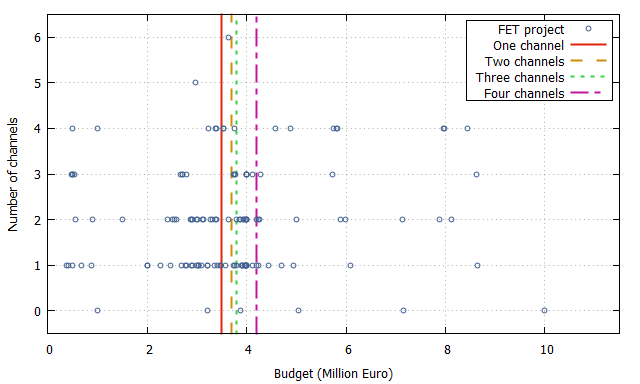
\includegraphics[scale=0.4]{Images/Channel_budget.png}
 \caption{Projects' distribution as a function of the available budget and of the number of considered online communication channels. The vertical lines are the budget medians of the group of projects with activated channels ranging between one and four. For the sake of clarity, the figure shows the budget range up to \euro 11.5 Million. The following projects were used for the medians calculation but lie outside the plotted budget range: QuantERA (\euro 40.5 Million, 3 channels), FLAG-ERA II (\euro 18.3 Million, two channels) and DEEP-EST (\euro 15.9 Million, 3 channels).}
 \label{Channel_budget}
 \end{center}
\end{figure}

The plot shows that the majority of the projects has activated a number of channels between one and four. Hence, four groups of projects were identified based on the amount of activated channels (from one to four). The other projects were not considered for the analysis presented in this section due to their limited number. For each of the four groups, the median of the corresponding projects' budgets was calculated. The median was preferred to the arithmetic mean as it is a more robust indicator in the presence of outliers. The values are reported in table \ref{Median} and drawn as vertical lines in figure \ref{Channel_budget}. 

The analysis suggests a weak correlation between the number of activated channels and the available budget. On one hand, the larger the median, the higher the number of channels. On the other hand, the variation between the median values are of the order of percent. Moreover, it must be borne in mind the the budget data corresponds to the total available funding, and not to the fraction allocated for communication purposes. Hence, in absolute terms of funds, and remembering that budgets are distributed over the project's duration (some years), the differences are not significantly large. The result indicates that the decision on the number of channels to open for a given project is not strongly influenced by the available budget, but rather on the pursued communication strategy. 

\begin{table}[t]
 \begin{center}
  \begin{tabular}{cc}
   \hline 
   \hline
   Number of channels & Budget median \\ 
   \hline
   \hline
   One & 3.4 \\
   Two & 3.5 \\
   Three & 3.8 \\
   Four & 4.0 \\
   \hline
   \hline
  \end{tabular}
 \end{center} 
 \caption{Medians of the projects' budgets as a function of the number of channels considered by the projects. Values are rounded and expressed in million Euros.}
\label{Median} 
\end{table}

\section{Budget impact: the case of the HPC and QT projects} \label{Budget_impact_the_case_of_the_HPC_and_QT_projects}
The approach followed in section \ref{Budget_impact} enabled a further comparison of QT and HPC projects. Figure \ref{Channel_budget_breakdown} shows the two classes as a function of the number of activated channels and available budget. Typically, QT projects lie in the range between \euro 2 and \euro 4 Million and have one active channel. HPC projects in the same budget window have considered more communication platforms. The result highlights the different communication strategy followed by the two classes of projects, as mentioned in section \ref{Online_presence_breakdown}. 

\begin{figure}[!t] 
 \begin{center}
 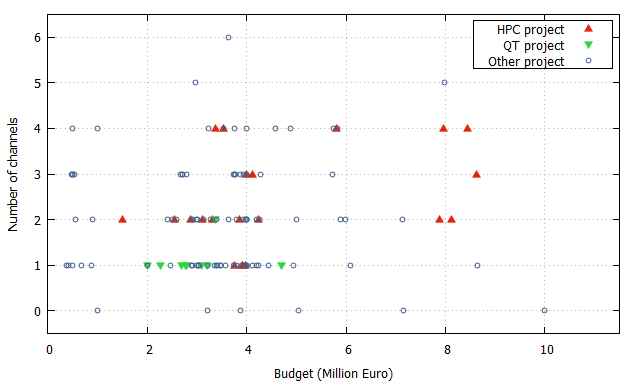
\includegraphics[scale=0.4]{Images/Channel_budget_breakdown.png}
 \caption{Distribution of HPC and QT projects as a function of the available budget and of the number of considered online communication channels. For the sake of clarity, the figure shows the budget range up to \euro 11.5 Million. The QuantERA project (\euro 40.5 Million, 3 channels) lies outside the plotted budget range.}
 \label{Channel_budget_breakdown}
 \end{center}
\end{figure}

\section{Chapter summary} 
In this chapter, the following items have been discussed:

\begin{enumerate}
 \item FET projects make use of several online communication channels. The most used channels are websites, twitter and facebook. Only a limited fraction of projects is active on YouTube and ResearchGate.
 \item The number of considered channels depends strongly on the class of FET project. HPC projects are among the most active initiatives. On the contrary QT project have very limited presence on the social platforms considered for this thesis.
 \item In general, the available budget has a limited impact on the number of active channels. Thus, the amount of social platforms considered by projects depend mainly on the pursued communication strategy.
 \item The guideline in the previous point holds for the HPC and QT classes. Selecting projects within similar budget ranges shows that the two sub-groups tend to follow opposite strategies. In general, HPC projects are active on several channels, whereas QT initiatives limit their online communication to the use of the website.       
\end{enumerate}